\documentclass{article}
\usepackage[a4paper, total={6in, 8in}, margin=20mm]{geometry}
\usepackage{graphicx}
\usepackage{hyperref}
\parindent=0pt
\parskip=12pt

\begin{document}
	The OPTIMADE API enables a user to obtain material information from multiple providers with the same filter query. This is particularly useful for machine learning workflows. Being able to query multiple providers using a single API allows one to combine data from multiple sources, with different ``strengths''. We demonstrate the same with an example, described below.
	
	We used the OPTIMADE API to get high-entropy alloy materials using the filter query 
	\begin{quote}
		`elements HAS ANY ``W",``Al",``Cd",``Zn" AND NOT elements HAS ANY ``B", ``Cl", ``F", ``H", ``N", ``O", ``S", ``Se" AND nelements$>$=5'		
	\end{quote}
	from three different providers (anonymized as P1, P2, P3). The number of materials returned by each provider and a Venn diagram of the sets of unique elements that appear in the materials from each provider are shown in the bottom inset in \autoref{fig: exampleFig}.

	Standard structural entries of the OPTIMADE specification, \verb|species_at_sites| and \verb|lattice_vectors| are used to calculate the density of the materials. Vectors codifying the composition of each material are also constructed. These vectors are used as the inputs to machine learning models which is trained to predict the densities (output). The dataset obtained using OPTIMADE is split into training and testing sets (80-20 split) while ensuring that proportional of entries from each provider remains the same in both training and testing sets.

	We choose a Random Forest Regressor (from the \verb|scikit-learn| package in Python) as the machine learning  for our example. We show that when this model is trained on data from all the providers, it performs much better (R$^2 = 0.98$, see top inset in \autoref{fig: exampleFig}) than when it is trained on data from only one data set when tested on data from the same pool. On the other hand, if data from a only one provider is used to training, as expected, the performance is much worse. We can see the loss of predictive power from the graph of predicted and actual density values in \autoref{fig: exampleFig}. For models trained only on data from a single provider, the prediction is quite accurate when tested on data from the same provider (indicted by `cross' markers). However, most of the predictive power is lost when tested on data from another provider (`dot' markers). Meanwhile, the model trained on data from call providers (C) retains its predictive power for data from all the providers.

	\begin{figure}[h]
		\centering
		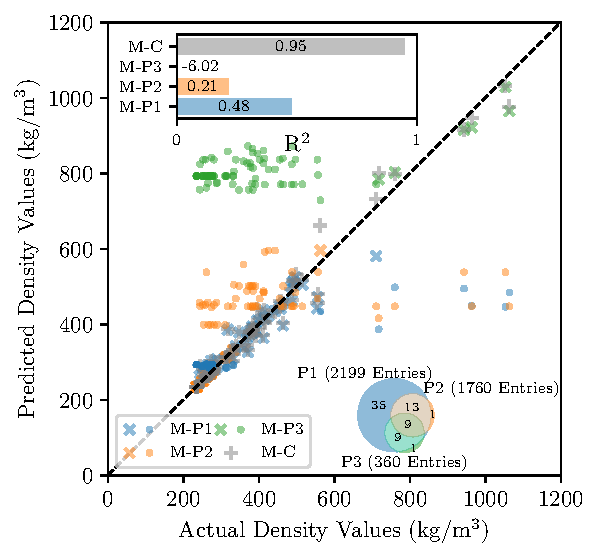
\includegraphics[]{scatterPlot.pdf}
		\caption{} 
		\label{fig: exampleFig}
	\end{figure}
\end{document}